\chapter{Estado de la Realidad Aumentada}

El campo de la Realidad Aumentada está en una continua y rápida evolución. En este capítulo se dará una pincelada de cual es el panorama actual en cuanto a tecnologías de deasrrollo y sus aplicaciones.

\section{Tecnologías y dispositivos}

Ya se vio en el capítulo de introducción una de las tecnologías disponibles para el desarrollo de software \textit{RA}, \textit{ARCore}, pero no es ni de lejos la única. \textbf{Apple} es uno de los agentes que más está apostando por la Realidad Aumentada en los últimos años para sus productos \textit{iPhone} y \textit{iPad}. \textbf{ARKit}\cite{arkit} es el framework que la compañia desarrolló para la creación de aplicaciones \textit{RA} para estos dispositivos. Utiliza el lenguaje \textit{Swift}. En sus primeras versiones se limitaba a la detección de superficies horizontales, pero con los años se han ido añadiendo funciones como la detección de imágenes, superficies verticales, e incluso \textit{oclusión ambiental}, gracias a la cual objetos del mundo real pueden superponerse a objetos digitales, tapándolos en parte o por completo. Al ser la propia empresa la manufacturadora del hardware lo conocen muy bien y han sabido optimizar el rendimiento y precisión de esta tecnología obteniendo resultados muy buenos.

\textbf{SimpleCV}\cite{simplecv} es otro framework muy usado. No está tan directamente enfocado a la \textit{RA} como los ejemplos anteriores, si no más bien a la visión por computador en general. Está basado en \textit{OpenCV}, una librería de bajo nivel para el mismo propósito. Una de las bazas que tiene es que se puede desarrollar en Java, C++ o Python.

\textbf{Vuforia}\cite{vuforia} es otro potente motor. Como puntos destacables, se pueden crear facilmente botones y menús interactuables desde un escenario de Realidad Aumentada y permite añadir oclusión ambiental. Además incluye también soporte para las \textit{Microsoft HoloLens} y el motor de videojuegos \textit{Unity}.

En cuanto a dispositivos, hasta ahora se han discutido sobre todo dispositivos móviles pero realmente cualquier sistema con una cámara tiene potencial para ser usado en \textit{RA}. Por ejemplo una webcam en un ordenador de sobremesa o un portátil. \textbf{HoloLens 2}\cite{hololens} (figura \ref{fig:hololens}) es otro ejemplo ejemplo, una suerte de gafas que su creadora \textit{Microsoft} define como un \textit{dispositivo holográfico} con aplicaciones preparadas para aumentar la precisión y productividad de las empresas. Estas cuentan con dos pantallas o \textit{lentes holográficas transparentes} a través de las cuales se muestra el contenido en 3D. Tiene \textit{eye tracking}, \textit{hand tracking}, cámara incorporada, micrófono y altavoces que se integran para intentar sumergir más al usuario en la experiencia. Usa una versión especial de \textit{Windows 10} como sistema operativo.

Otra propuesta son las \textbf{Apple Vision Pro} (figura \ref{fig:visionpro}) , un dispositivo similar a las \textit{HoloLens 2} pero enfocado más al ámbito casero que al empresarial. Fueron presentadas en junio de 2023 y a fecha de este trabajo todavía no se han puesto a la venta, por lo que no se tiene mucha información.

\begin{figure}[h]
    \centering
    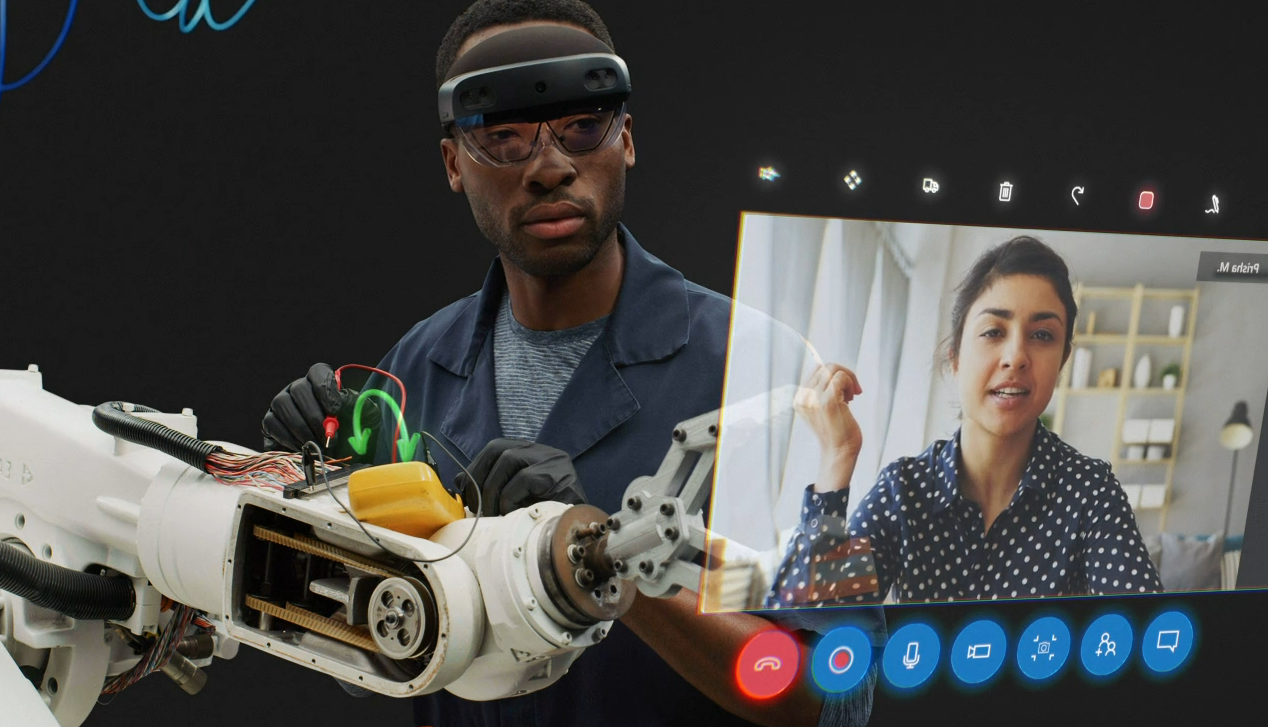
\includegraphics[scale=0.2]{hololens}
    \caption[HoloLens 2]{Concepto de gafas HoloLens 2 de Microsoft asistiendo a un ingeniero en un taller de robótica}
    \label{fig:hololens}
\end{figure}

\begin{figure}[h]
    \centering
    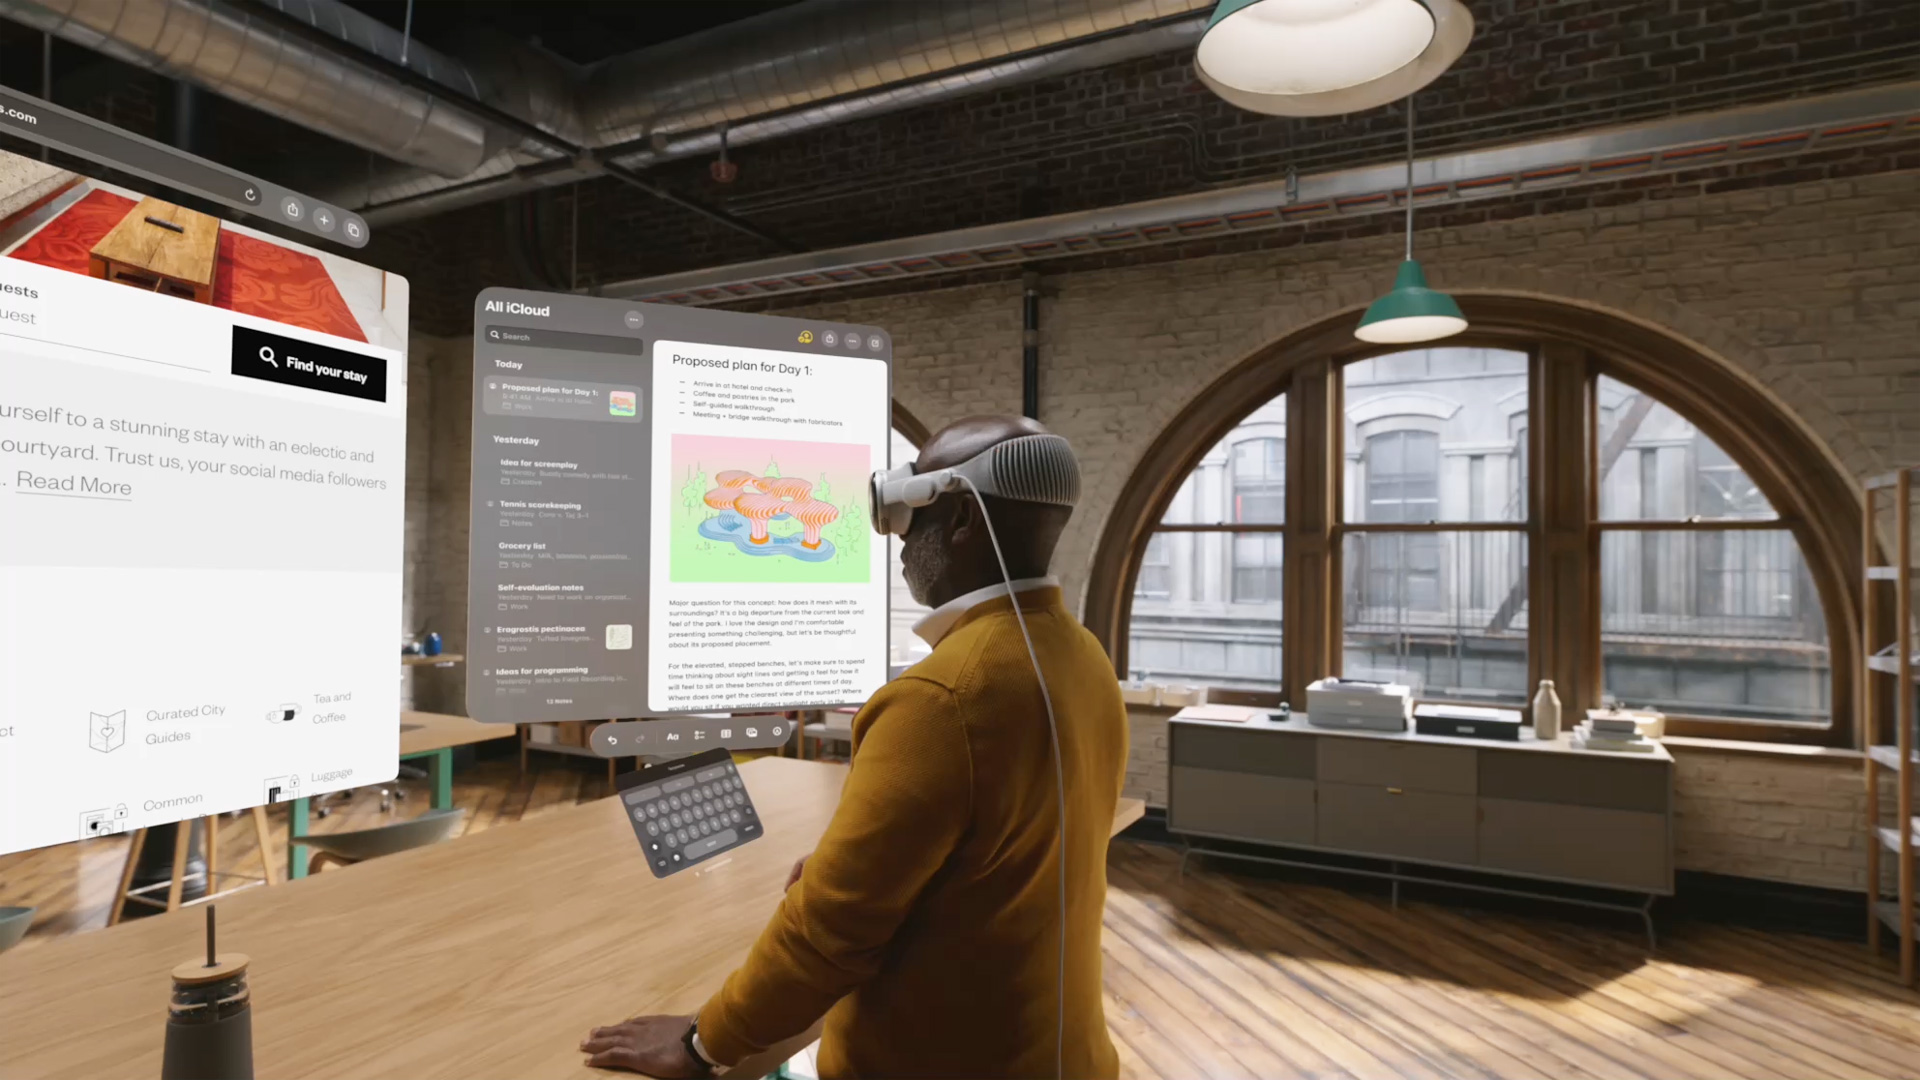
\includegraphics[scale=0.13]{applevision}
    \caption[Apple Vision Pro]{Concepto de gafas Apple Vision Pro sustituyendo el uso de un ordenador de sobremesa}
    \label{fig:visionpro}
\end{figure}

\section{Aplicaciones}

\subsection*{Videojuegos y juguetes}

El uso de la Realidad Virtual en los videojuegos se remonta a 2003 con \textit{Eye Toy}\cite{eyetoy}, una webcam lanzada por \textit{Sony} para su videoconsola Playstation 2. Esta se lanzó con juegos que detectaban el movimiento de usuario permitiendole interactuar con un entorno de imágenes planas superpuesto.

Otros ejemplos más actuales son los juegos \textit{RA} basados en posicionamiento como \textit{Ingress}, \textit{Pokémon Go} o \textit{Pikmin Bloom}. En estos los jugadores atienden a lugares concretos del mundo real con sus \textit{smartphones} para tomar parte en eventos como capturar criaturas, conquistar territorios o cultivar plantas, todo ello apoyado de la tecnología \textit{RA} para integrar estas actividades en el mundo real.

También existen juguetes radiocontrol como \textit{Mario Kart Live} (figura \ref{fig:mario})  en el que se usan elementos físicos para definir la trayectoria de un circuito de carreras en una habitación y posteriormente correr carreras con un coche con cámara integrada. A través de la pantalla se ven elementos añadidos como objetos y otros participantes. El coche interactúa con estos elementos. Si choca contra un obstáculo virtual, frenará.

\begin{figure}[h]
    \centering
    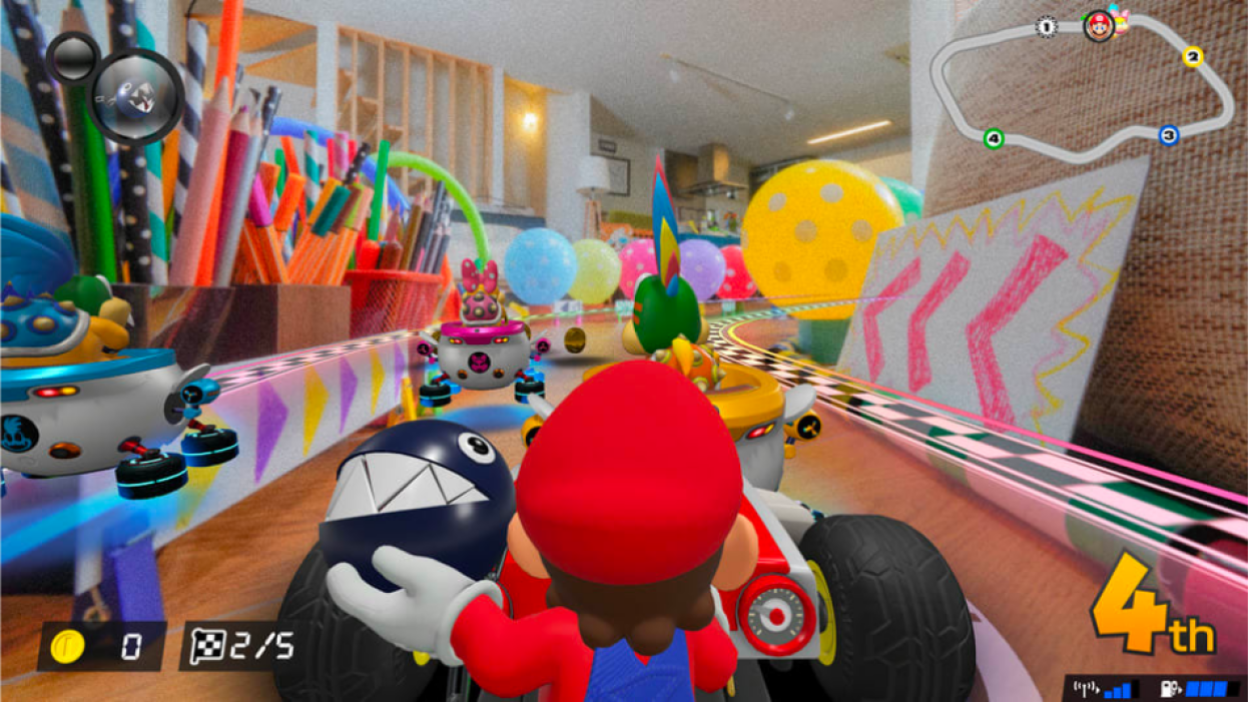
\includegraphics[scale=0.20]{mario}
    \caption[Mario Kart Live]{Juguete radiocontrol Mario Kart Live superponiendo un circuito virvual en uno físico.}
    \label{fig:mario}
\end{figure}

\subsection*{Uso comercial y marketing}

Esta tecnología es muy vistosa y que puede llamar facilmente la atención a personas que no mantengan mucho contacto con ella. Es por eso que es una herramienta muy potente para hacer campañas de márketing. En \cite{agtech} se relata como en 2008 la casa de automóviles \textit{MINI} lanzó una campaña en algunas revistas de automovilismo alemanas en la que el usuario podía ver un modelo 3D de un coche sobre la revista al enfocarla con una webcam.

La Realidad Virtual también ofrece soluciones a la hora de construir prototipos. Una maqueta industrial es algo caro de producir, pero necesario para valorar si un producto necesita más ajustes antes de ser lanzado al mercado. Y este suele ser el caso, lo que implica fabricar nuevos prototipos que cuestan todavía más dinero. Un grupo del \textit{nstitute of Industrial Technologies and Automation (ITIA)} del \textit{National Council of Research (CNR)} desarrollaron sistemas de \textit{AR} y \textit{VR} para soportar prototipado virtual \cite{agtech}.

\subsection*{Medicina}

Un uso muy extendido de la \textit{RA} en medicina es en la representación de imágenes para la cirugía guiada. Cuando se va a realizar una operación se realizan estudios en el paciente tales como \textit{CT} (Computer Tomography) o escaneos \textit{MRI} (Magnetic Resonance Imaging). Estos procesos generan recursos visuales a través de los cuales se planea la cirugía. Posteriormente se genera un modelo 3D a partir de estos recursos de los estudios pre operatorios. Este modelo puede proyectarse con Realidad Aumentada sobre el cuerpo del paciente para una mejor referencia en la sala de operaciones pudiendo mejorar así el rendimiento y las probabilidades de éxito.\cite{arintro}

\begin{figure}[h]
    \centering
    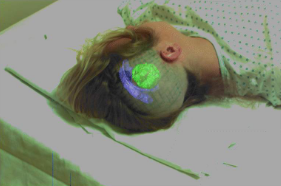
\includegraphics[scale=0.60]{operation}
    \caption[Cirugía guiada por imágenes]{Cirugía guiada por imágenes sobre el cuerpo de un paciente.}
    \label{fig:operation}
\end{figure}